
\begin{figure}
  \centering
  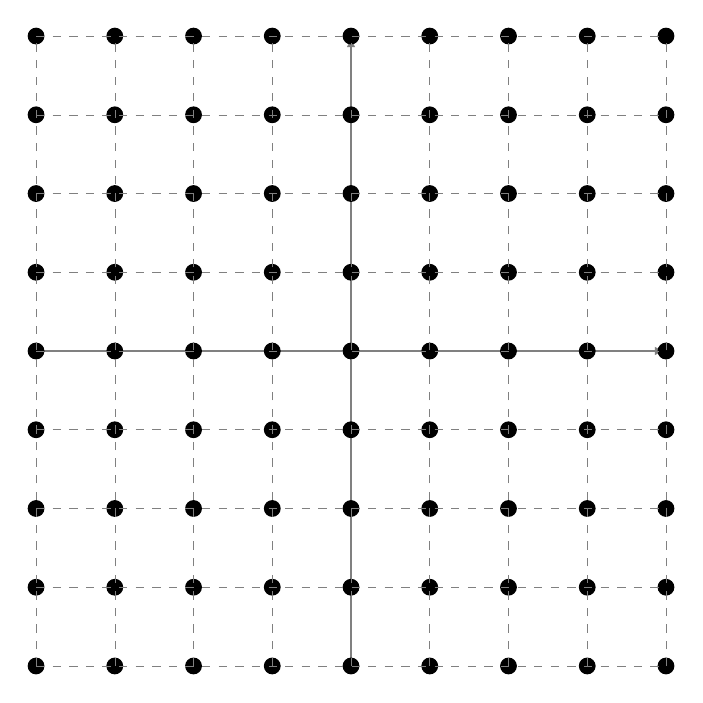
\begin{tikzpicture}[scale=1]
    \coordinate (Origin)   at (0,0);
    \coordinate (XAxisMin) at (-4,0);
    \coordinate (XAxisMax) at (4,0);
    \coordinate (YAxisMin) at (0,-4);
    \coordinate (YAxisMax) at (0, 4);
    \draw [thin, gray,-latex] (XAxisMin) -- (XAxisMax);% Draw x axis
    \draw [thin, gray,-latex] (YAxisMin) -- (YAxisMax);% Draw y axis

    %\clip (-3,-2) rectangle (10cm,10cm); % Clips the picture...
    \pgftransformcm{1}{0}{0}{1}{\pgfpoint{0cm}{0cm}}
          % This is actually the transformation matrix entries that
          % gives the slanted unit vectors. You might check it on
           % MATLAB etc. . I got it by guessing.
          % Draws a grid in the new coordinates.
    \foreach \x in {-4,-3,...,4}{% Two indices running over each
      \foreach \y in {-4,-3,...,4}{% node on the grid we have drawn 
        \node[draw,circle,inner sep=2pt,fill] at (\x,\y) {};
            % Places a dot at those points
      }
    }
    \draw[style=help lines,dashed] (-4,-4) grid[] (4,4);
  \end{tikzpicture}
  \caption{Vector Space $\R^2$ for $\forall (x,y); -4 \leq x \leq 4 and -4 \leq y \leq 4$.}
  \label{figure:solving-CVP-bad-basis}
\end{figure}
